
\noindent\begin{minipage}{\textwidth}
    \begin{table}[H]
        \centering
        \caption{Hiperparâmetros e Resultados do Melhor Modelo - densenet\_v9\_AM\_opt\_aug}
        \vspace{0.2cm}
        \resizebox{\textwidth}{!}{%
            \begin{tabular}{ll | lrrr}
                \hline
                \multicolumn{2}{c|}{\textbf{Hiperparâmetros}} & \multicolumn{4}{c}{\textbf{Métricas por Classe}} \\ \hline
                \textbf{Parâmetro} & \textbf{Valor} & \textbf{Classe} & \textbf{Precisão} & \textbf{Recall} & \textbf{F1-Score} \\ \hline
    Agendador (Patience) & 3 & 31.2 & 0.7384 & 0.7743 & 0.7559 \\ 
Agendador de LR & ReduceLROnPlateau & 31.3 & 0.6333 & 0.7525 & 0.6878 \\ 
Architecture & densenet121 & 31.4 & 0.5391 & 0.6238 & 0.5784 \\ 
Batch Size & 32 & 32.3 & 0.7554 & 0.7092 & 0.7316 \\ 
Data Augmentation & False & 32.4 & 0.9600 & 0.4138 & 0.5783 \\ 
Decaimento de Peso (WD) & 0.0002 & 33.3 & 0.6227 & 0.7098 & 0.6634 \\ 
Dropout & 0.2763 & 41.4 & 0.7391 & 0.3864 & 0.5075 \\ 
Função de Perda & CrossEntropyLoss & 41.5 & 0.8333 & 0.7692 & 0.8000 \\ 
Hidden Units & 256 & 42.4 & 0.8235 & 0.4118 & 0.5490 \\ 
Label Smoothing & 0.1000 & 44.4 & 0.8696 & 0.6897 & 0.7692 \\ 
\cline{3-6} 
Otimizador & AdamW & \textbf{Média (Macro)} & 0.7749 & 0.6581 & 0.6971 \\ 
Taxa de Aprendizado (LR) & 2.95e-04 & \textbf{MCC} & \multicolumn{3}{c}{0.6504} \\ 
Unfreeze Layers & 6 &  & & &  \\ 
            \hline
            \end{tabular}%
        }
    \end{table}

    \begin{figure}[H]
        \centering
        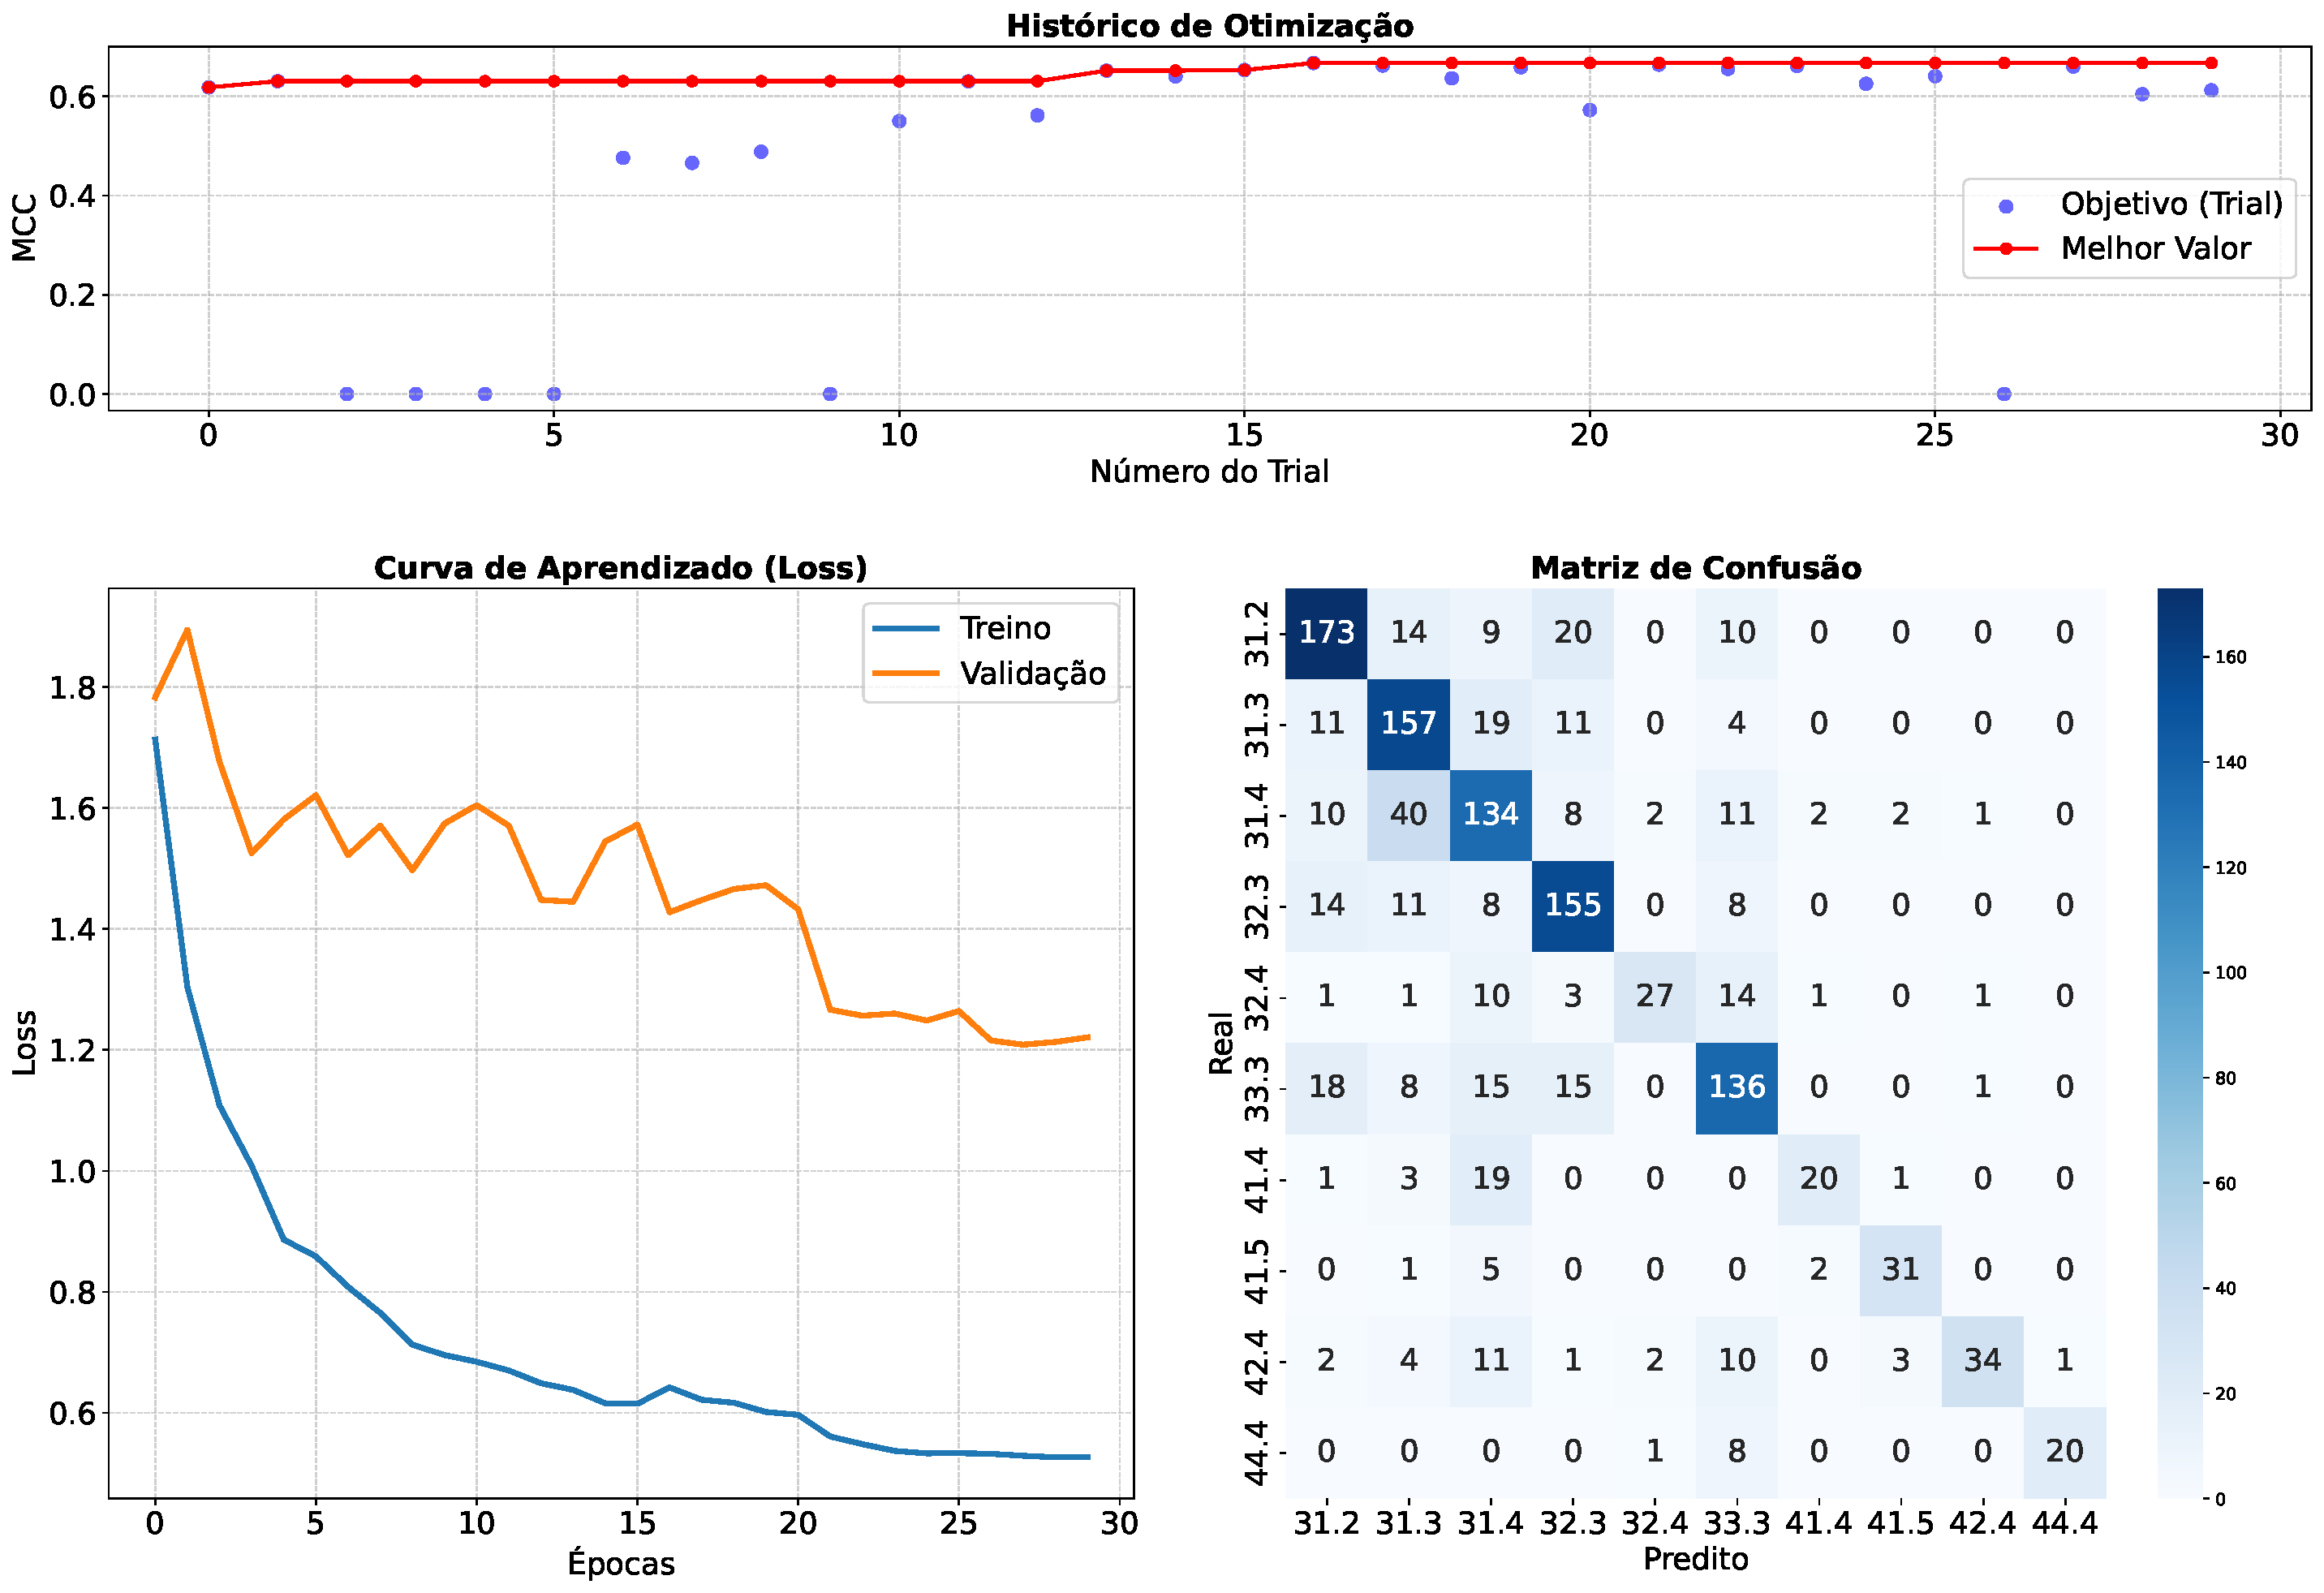
\includegraphics[width=0.85\textwidth]{tex/appendix/experiments/densenet_v9_AM_opt_aug/dashboard_consolidado.pdf}
        \caption{Histórico de Otimização, Curvas de Aprendizado e Matriz de Confusão - densenet\_v9\_AM\_opt\_aug}
    \end{figure}
\end{minipage}
\clearpage
